\documentclass[twocolumn, 10pt]{article}
\usepackage{amsmath,amsthm,amssymb,wrapfig,graphicx}
\begin{document}
\section{Fundamental}
28 May 2023
\subsection{Intervals}
Intervals are basically subsets of $\mathbb{R}$ and are commonly used in solving inequalities or in finding domains. If there are two numbers $a, b \in \mathbb{R}$ such that $a < b$, there are four types of intervals: 
\begin{itemize}
\item Open interval: $(a,b)=\{x:a<x<b\}$ i.e end points are not included. Symbols: $()$ or $][$
\item Closed interval: $[a,b]=\{x:a \le x \le b\}$ i.e end points are also included. Symbol: $[ \thinspace]$
\item Open-Closed interval: $(a,b)=\{x:a<x \le b\}$. Symbols: $( \thinspace ]$ or $]\thinspace]$
\item Closed-Open interval: $(a,b)=\{x:a \le x <b\}$. Symbols: $[ \thinspace )$ or $[\thinspace[$
\end{itemize}
\textbf{Infinite Intervals}
\begin{itemize}
\item $(a,\infty)= \{x:x>a\}$
\item $[a,\infty)=\{x:x \ge a\}$
\item $(-\infty,b)=\{x:x<b\}$
\item $(\infty,b]=\{x:x \le b\}$
\item $(-\infty,\infty)=\{x:x \in \mathbb{R}\}$
\end{itemize}
\subsection{Sets and Relations}
\subsubsection{Set}
 A collection of any kind of objects. The objects that make  up a set are called $elements$ or $members$. The statement '$a$ is an element of set $A$' can be written as $a \in A$ and set containing elements $a,b$ and $c$ is denoted by $\{a,b,c\}$. A $empty$  or $null$ set is denoted by  $\varnothing$, which is the set that contains no elements.\\
\textbf{Union(join,sum):} The union of two sets $A$ and $B$, denoted by $A \cup B$, consists of those elements that belong to $A$ or to $B$: $$A \cup B = \{x:(x \in A) \lor (x \in B)\}$$ For example, if $A$ is $\{1,2,3,4\}$ and $B$ is $\{1,4,5,6\}$ then $A \cup B$  is $\{1,2,3,4,5,6\}$.\\
\textbf{Intersection(meet,product):} The intersection of two sets $A$ and $B$, denoted by $A \cap B$, consists of those elements that belong to both $A$ and $B$: $$A \cap B=\{x:(x \in A) \land (x \in B)\}$$ For example, if $A$ is $\{1,2,3,4,5,6\}$ and $B$ is $\{1,4,5,6,7,8\}$ then $A \cap B$ is $\{1,4,5,6\}$.\\
\textbf{Complement:} The complement of a set $A$, denoted by $A'$ or $A^{\complement}$, consists of all those elements that are not members of $A$: $$A'=\{x:x \not \in A\}$$ For example, in the domain of natural numbers, if $A$ is set of even numbers the its complement $A'$ is the set of odd numbers.\\
\textbf{Universal Set:} Relative to a particular domain, the universal set, denoted by $\mathbf{U}$, is set of all objects of that domain:
$$\mathbf{U}=\{x:x=x\}$$
\subsubsection{Properties of sets}
\textbf{Commutative law:}
\begin{itemize}
\item $(A \cup B)=B \cup A$
\item $(A \cap B)= B \cap A$
\end{itemize}
\textbf{Associative law:}
\begin{itemize}
\item $(A \cup B) \cup C=A \cup (B \cup C)$
\item $(A \cap B) \cap C=A \cap (B \cap C)$
\end{itemize}
\textbf{Distributive law:}
\begin{itemize}
\item $A \cup (B \cap C)=(A \cup B) \cap (A \cup C)$
\item $A \cap (B \cup C)=(A \cap B) \cup (A \cap C)$
\end{itemize}
\textbf{De Morgan's law:}
\begin{itemize}
\item $(A \cup B)' = A' \cap B'$
\item $(A \cap B)' = A' \cup B'$
\end{itemize}
\textbf{Identity law:}
\begin{itemize}
\item $A \cup \mathbf{U}=A$
\item $A \cup \varnothing=A$
\end{itemize}
\textbf{Complement law:}
\begin{itemize}
\item $A \cup A' = \mathbf{U}$
\item $A \cap A'= \varnothing$
\item $(A')'=A$
\end{itemize}
\textbf{Idempotent law:}
\begin{itemize}
\item $A \cap A=A$
\item $A \cup A=A$
\end{itemize}
\subsubsection{Results on number of elements in sets}
If $A,B,C$ are finite sets and $\mathbf{U}$ be Universal finite set then:
\begin{itemize}
\item $n(A \cup B)= n(A) + n(B) -n(A \cap B)$
\item $n(A-B)=n(A)-n(A \cap B)$
\item $n(A \cup B \cup C)=n(A)+n(B)+n(C)-n(A \cap B)-n(B \cap C)-n(C \cap A)+n(A \cap B \cap C)$
\end{itemize}
\subsubsection{Relations}
An association between, or property of, two or more objects. Thus ($x=y$) and ($a$ lies between $b$ and $c$) are relations, but ($N$ is a prime) is not.
\subsubsection{Types of Relations}
\textbf{Void Relation:} Let $A$ be a set. Then $\phi \subseteq A \times A$ and so it is a relation on $A$. This relation is also called empty relation on $A$.\\
\textbf{Universal Relation:}Let $A$ be a set. Then $A\times A \subseteq A \times A$ and so it is a relation on A. This relation is called the universal relation on $A$.\\
\textbf{Identity relation:} Let $A$ be a set. Then the relation $I_A =\{(a,a):a \in A\}$is called the identity relation on $A$. In other words, a relation $I_A$ on $A$ is called the identity relation if every element of $A$ is related to itself only.\\
\textbf{Reflexive Relation:} A relation $R$ on a set $A$ is said to be reflexive if every element of $A$ is related to itself. Thus $R$ on set $A$ is not reflexive if there exits an element $a \in A$ such that $(a,a) \notin R$.\\
\textbf{Symmetric Relation:} A Relation $R$ on set $A$ is said to be symmetric if $$(a,b) \in R \implies (b,a) \in R \medspace \forall \medspace a,b \in A$$ i.e $$a \medspace R \medspace b \implies b \medspace R \medspace a \medspace \forall \medspace a,b \in A$$\\
\textbf{Transitive Relation:} A Relation $R$ on set $A$ is said to be transitive  if $(a,b) \in R$ and $(b,c) \in R$ $\implies (a,c) \in R \medspace \forall \medspace a,b,c \in A$.\\
\textbf{Equivalence Relation:} A Relation is said to be equivalence if it satisfies $reflexive,symmetric$ and $transitive$ relations.\\
\textbf{Equivalence Class:} If $R$ is an equivalence relation defined on set $A$ then the equivalence class of any element $x \in A$, denoted by $[x]$, is the set of elements to which $x$ is related by equivalence relation $R$: $$[x]=\{y:x \medspace \mathbf{R} \medspace y\}$$ For example, if $R$ is the equivalence relation (the same height as), then the equivalence class of the element $x \in A$ consists of all elements of $A$ with same height as $x$.
\section{Quadratic Equations}
29 May 2023
\subsection{Equation and Basic Results}
An equation of the form $$ax^2+bx+c=0$$ where $a \not= 0$ and $a,b,c \in \mathbb{R}$ is called a quadratic equation. The roots of quadratic equation are given by $$x=\frac{-b \pm \sqrt{b^2-4ac}}{2a}$$ The quantity D ($D=b^2-4ac$) is known as discriminant of equation.
\subsubsection{Results}
1. Let $\alpha$ and $\beta$ be two roots of given quadratic equation. Then

\begin{itemize}
\item $\alpha + \beta = -\frac{b}{a}$
\item $\alpha \beta=\frac{c}{a}$
\end{itemize}
2. A quadratic equation, whose roots are $\alpha$ and $\beta$ can be written as $$(x-\alpha)(x-\beta)=0$$ i.e $$ax^2+bx+c \equiv a(x-\alpha)(x-\beta)$$
3. If the quadratic equation is satisfied by more than two distinct numbers (real or complex), then it becomes an identity, i.e $$a=b=c=0$$
4. The quadratic equation has real and equal roots if and only if $D=0$ i.e $b^2-4ac=0$. \\
5. The quadratic equation has real and distinct roots if and only if $D>0$ i.e $b^2-4ac>0$. \\
6. The quadratic equation has complex roots with non-zero imaginary parts if and only if $D<0$ i.e $b^2-4ac<0$.\\
7. If $p+iq$ ($p,q \in \mathbb{R}$) is root of quadratic equation where $i=\sqrt{-1}$, the $p-iq$ is also root of quadratic equation. Provided $a,b,c \in \mathbb{R}$. \\
8. If $p+\sqrt{q}$ is an irrational root of quadratic equation, then $p-\sqrt{q}$ is also a root of equation provided that all coefficients are rational.
\subsection{Conditions for Common Root(s)}
Let $ax^2+bx+c=0$ and $dx^2+ex+f=0$ have a common root $\alpha$. Then 
$a\alpha ^{2}+b\alpha+c=0$ and $d\alpha ^{2}+e\alpha+f=0$.\\
Solving for $ \alpha^2$ and $ \alpha$ :
$$\frac{\alpha^2}{bf-ce}=\frac{\alpha}{dc-af}=\frac{1}{ae-bd} \implies$$ $$\alpha^2=\frac{bf-ce}{ae-bd}$$ and $$\alpha=\frac{dc-af}{ae-bd} \implies$$ $$(dc-af)^2=(bf-ce)(ae-bd)$$
which is a required condition for the two equation to have a common root.

\begin{itemize}
\item Condition for both the roots to be common is $\frac{a}{d}=\frac{b}{e}=\frac{c}{f}$
\end{itemize}
\subsection{Wavy Curve Method}
The Method of intervals is used for solving inequalities of the form 
$$f(x)= \frac{(x-a_1)^{n_1}(x-a_2)^{n_2}...(x-a_k)^{n_k}}{(x-b_1)^{m_1}(x-b_2)^{m_2}...(x-b_p)^{n_p}} >0(<0, \le 0, or \ge 0 )$$
where $n_1,n_2,n_3...n_k$, $m_1,m_2,m_3..m_p$ $\in \mathbb{N}$ and the numbers $a_1,a_2,...a_k$, $b_1,b_2,...b_p$ $\in \mathbb{R}$ such that
$a_i \not= b_i$ where $i=1,2,3,...k$ and $j=1,2,3,...p$.\\
\textbf{Statements}
\begin{itemize}
\item All $zeros^1$ of the function $f(x)$ contained on left hand side of the inequality should be marked on the number line with black circles.
\item All points of $discontinuities^2$ of the function $f(x)$ contained on left hand side of the inequality should be marked with white circles.
\item Check the value of $f(x)$ for any real number greater than the right most marked number on the number line. 
\item From right to left, beginning above the number line, a wavy curve should be drawn which passes through all the marked points so that when passes through $single \medspace point^3$, the curve intersects the number line, and when passing through a $double \medspace point^4$, the curve remains located on the one side of number line.
\item The appropriate intervals are chosen in accordance with sign of inequality. Their union just represents the solution of inequality.
\end{itemize}
\textbf{Remarks}
\begin{itemize}
\item The points of discontinuity will never be included in answers.
\item $Zeros^1$:The point for which $f(x)$ vanishes(becomes zero) is called the $zeros$ of function e.g. $x=a_i$
\item $Discontinuities^2$:The points $x=b_j$ are the points of the $discontinuity$ of the function.
\item $Single \medspace point^3$:If the exponents of factor is $odd$ then the point is called $single \medspace point$.
\item $Double \medspace point^4$: If the exponent of factor is $even$ then the point is called $double \medspace point$.
\end{itemize}
\subsection{Quadratic Expression}
Let $f(x)=ax^2+bx+c$ where $a,b,c \in \mathbb{R}$ $a \not= 0$
It can be rewritten as $$f(x)=a\{(x+ \frac{b}{2a})^2 + \frac{D}{4a^2}\}$$ where $D=b^2-4ac$. Then $y-f(x)$ represents a parabola whose axis is parallel to the y axis, with vertex at $A(-\frac{b}{2a},\frac{-D}{4a})$. Now depending upon the values of $a$ and $D$ the parabola will have different shapes:

\begin{wrapfigure}{R}{0.3\textwidth}
\centering
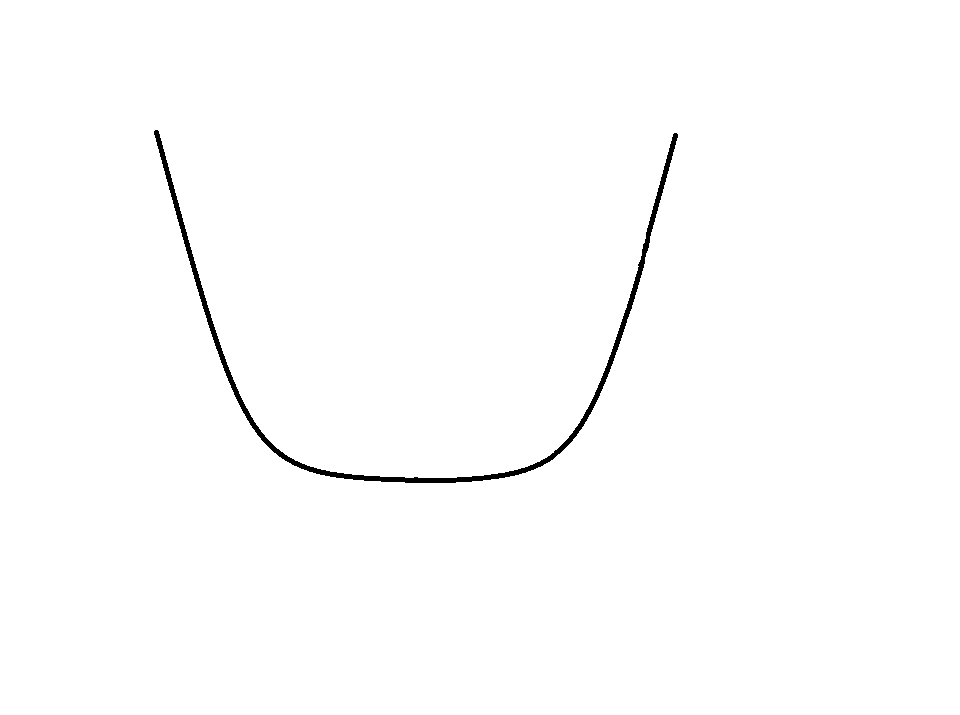
\includegraphics[width=0.25\textwidth]{images/parabola.png}
\caption{\label{fig:check} $y=4ax^2$ Trial figure}
\end{wrapfigure}
\end{document}